%!TEX root = ../Bachelorarbeit.tex
\chapter{Data-centric Design}
\label{sec:dcd}
In diesem Kapitel wird die grundlegende Architektur der Anbindung eines persistenten Speichers im Core von Project-Zoom näher erläutert. Das gewählte Design hat vorrangig Auswirkungen auf die Art und Weise, wie der Code für Datenmodelle geschrieben wird, erstreckt sich aber als Betrachtungsweise über die gesamte Architektur. Zuerst wird das verwendete Data Centric Design näher beschrieben und mit alternativen etablierten Formen der Datenbankanbindung verglichen. Anschließend wird näher auf die Umsetzung des Designs in Project-Zoom eingegangen

\section{Motivation}
\label{sec:dcdmotivation}
Das JSON Coast-To-Coast Design als Umsetzung des data-centric Designs wurde erstmals zusammenhängend und mit Beispielen unterlegt von Pascal Voitet dargestellt \cite{jctc}. Voitet ist selbst Mitwirkender am Open-Source-Projekt Play und Autor von Scala-Bibliotheken (\tete{play-reactivemongo}\footnote{\url{ https://github.com/zenexity/Play-ReactiveMongo}}, \tete{play-autosource}\footnote{\url{ https://github.com/mandubian/play-autosource}}). 

Ein Backend für eine Webapplikation ist zunehmend eine Verbindung zwischen verschiedenen anderen Backends und Frontends. Diese Entwicklung geht auf die Bereitstellung von APIs für viele große und kleine im Web verfügbare Dienste zurück. Anwendungen, welche Daten vorrangig aus anderen Quellen aggregieren, sind zum großen Teil mit der Datenmanipulation beschäftigt. Hier bietet sich ein data-centric Design an. Grundlegend für das Design sind dabei drei Entwicklungen: Zum einen das Aufstreben von NoSQL-Datenbanken und zum anderen asynchrone Datenbanktreiber mit einfachen Methoden zur JSON-Manipulation.

\subsection{NoSQL}
Die Entwicklung der Datenbankmanagementsysteme bestand viele Jahre lang in der Optimierung und Verbesserung bestehender relationaler Datenbankmodelle. Im Jahr 1998 kam der Term Not-only SQL (NoSQL) auf \cite{storage-solutions}. Heute gibt es verschiedene etablierte Datenbanken, die keine reinen SQL Datenbanken mehr sind, wie beispielsweise MongoDB, Apache CouchDB und Apache Cassandra\footnote{\url{http://cassandra.apache.org}}.

\subsection{Datenbanktreiber}
\label{sec:reactive}
Für die Anbindung von relationalen Datenbanken gibt es in Java die Java Database Connectivity (JDBC). Diese Schnittstelle abstrahiert über Datenbanken und deren Treiber, indem eine einheitliche API angeboten wird. Ausgerichtet ist JDBC auf relationale Datenbanken \cite{reese2000database}.

Um NoSQL-Datenbanken anzubinden, benötigt man, wie bei JDBC, einen eigenen Treiber. Der Unterschied ist, dass es hier keine Abstraktionsebene über verschiedene NoSQL-Datenbanken gibt. Dies liegt vorrangig an der sich stark unterscheidenden Struktur der einzelnen Speichersysteme. Die unterschiedlichen NoSQL-Datenbanken sind jeweils speziell auf eine bestimmte Aufgabe ausgerichtet, wie z.B. auf Durchsatz, verteilte Umgebungen oder flexible Datenschemas. 

\tete{ReactiveMongo} ist ein asynchroner Datenbanktreiber für MongoDB und die Programmiersprache Scala. Die Vorteile eines asynchronen Treibers liegen auf der Hand: Für jede synchrone Datenbankabfrage wird normalerweise ein Thread verwendet, der bis zur Antwort blockiert ist. Bei mehreren Datenbankabfragen pro Request werden bei Last viele Threads benötigt, um Datenbankabfragen auszuführen. Asynchrone Treiber umgehen dieses Problem, indem sie Threads, welche Datenbankabfragen ausführen, nicht blockieren. Für dieses Konzept ist es notwendig, Platzhalter einzuführen. Diese ersetzen das Ergebnis, solange es noch nicht vorhanden ist.

\begin{lstlisting}[label=lst:asyncaccess, caption=Funktionssignatur für asynchronen Datenbankzugriff]
def findOneById(bid: BSONObjectID): Future[Option[Graph]]
\end{lstlisting}
 
Im Quelltext \ref{lst:asyncaccess} zeigt die Funktionssignatur den Rückgabetyp \tete{Future[Option[Graph]]}. \tete{Future} ist hierbei ebendieser Platzhalter für ein Ergebnis, welches noch nicht existiert. Um auf das Ergebnis eines \tete{Futures} zu reagieren, können verschiedene \tete{Callbacks} festgelegt werden.


\subsection{Manipulation von JSON}
Das data-centric Design basiert auf der Idee der direkten Manipulation von Daten. Für eine Umsetzung des data-centric Designs mit Hilfe von JSON benötigt man somit eine Bibliothek, welche die Möglichkeit bietet, JSON zu transformieren und zu validieren.
 
Eine solche Bibliothek, welche das Validieren, Transformieren und Serialisieren erlaubt, ist Play-JSON. Ein Beispiel, wie solch eine Transformation und Validierung aussieht, ist im Anhang im Quelltextauszug \ref{app:jsonbsp} zu sehen. Dort wird ein JSON-Objekt erzeugt, welches anschließend zuerst transformiert wird, indem das Attribut \tete{role} angehangen wird, und danach validiert wird. Bei der Validierung wird überprüft, ob der Nutzer über 18 Jahre alt ist.

\section{Idee hinter data-centric Design}
Das Ziel im data-centric Design ist die direkte Manipulation von Daten. Der Fokus des Designs liegt dabei sowohl auf der Datenmanipulation als auch auf dem Datenfluss. Wie bereits im Abschnitt \ref{sec:dcdmotivation} beschrieben, sind Webapplikation Backends immer Häufiger Knotenpunkte in einem mehrere Server durchlaufenden Datenfluss. Ein Teil dieses Datenflusses, die Kommunikation des Backends mit der Datenbank und dem Client, ist in Abbildung \ref{fig:dataflow} dargestellt. 

\begin{figure}[h]   
  \centering     
  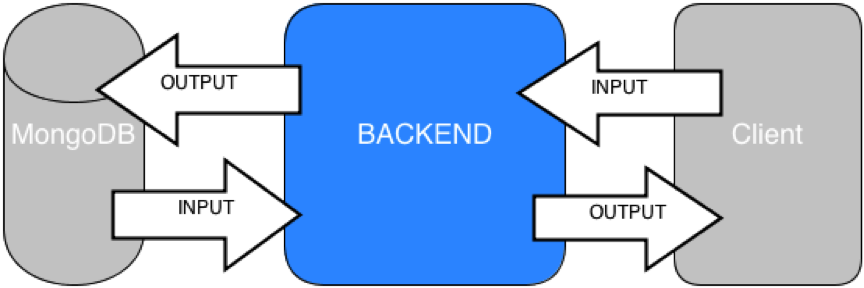
\includegraphics[width=0.8\textwidth]{img/dataflow.png}  
   \caption{Datenfluss zwischen Datenbank, Backend und Client}   
  \label{fig:dataflow} 
\end{figure}

In diesem Datenfluss soll es keine implizite Umwandlung der Daten in Objekte der Programmiersprache\footnote{Es ist bekannt, dass die Repräsentation der Daten des Datenflusses ebenfalls in Objekten der Programmiersprache erfolgt (beispielsweise JSON-Objekte). Mit dem Ausdruck ist die Überführung der Daten aus einem allgemeinen Modell (z.B. JSON) in eine spezifische Objektdarstellung (z.B. ein Objekt einer User-Klasse) gemeint.} geben. Für ein einfaches Durchleiten der Daten aus der Datenbank zum Client oder von einer anderen Webressource zum Client ist eine Umwandlung nicht notwendig oder sinnvoll. 

Im Gegensatz zu anderen Modellen ist die Abstraktion von der Datenquelle kein Ziel des data-centric Designs. Das Festlegen auf eine Datenquelle bei der Entwicklung eines Systems erlaubt die Verwendung aller Funktionen, die diese Datenquelle zur Verfügung stellt. Beispielsweise erlaubt MongoDB die Verwendung sogenannter \tete{Capped Collections}\footnote{Mehr Informationen zu Capped Collections z.B. auf \url{http://docs.mongodb.org/manual/core/capped-collections/}}, welche auf hohen Durchsatz optimiert sind. Diese verhalten sich wie eine zirkuläre Queue mit begrenzter Größe. Viele Datenbanken besitzen spezielle, stark angepasste Funktionen, auf die jedoch bei der Verwendung von allgemeinen Datenbank APIs (z.B. JDBC) meist nicht zugegriffen werden kann. Ein Nachteil dieser engen Kopplung ist, dass der Austausch der Datenquelle dadurch schwieriger ist. 

Eine Deserialisierung der Daten in Objekte ist für komplexe Business-Logik von Vorteil. Statische Datenmodelle sollten immer dann verwendet werden, wenn die Manipulation der Daten kompliziert wird oder wenn die Verwendung externer Bibliotheken eine Objektrepräsentation benötigt. 

Nach Voitet ist die Frage also nicht, statische Datenmodelle zu vergessen, sondern sie nur dann zu benutzen, wenn sie notwendig sind. Einfache und dynamische Strukturen sollten so oft es geht erhalten bleiben \cite{jctc}.

\section{Abgrenzung zur objektrelationalen Abbildung}
Das \tete{Object-relational Mapping} (ORM) bezeichnet man auch als \tete{All-Model-Approach}. Hierbei erfolgt die Kommunikation mit der Datenbankschnittstelle über Objekte der Programmiersprache. Abfragen an die Datenbank resultieren in Objekten der Programmiersprache. Der Fokus der objektrelationalen Abbildung liegt in der Überführung von Objekten der objektorientierten Programmierung in ein relationales, tabellenorientiertes Schema \cite{wambler}. 

\begin{figure}[h]   
  \centering     
  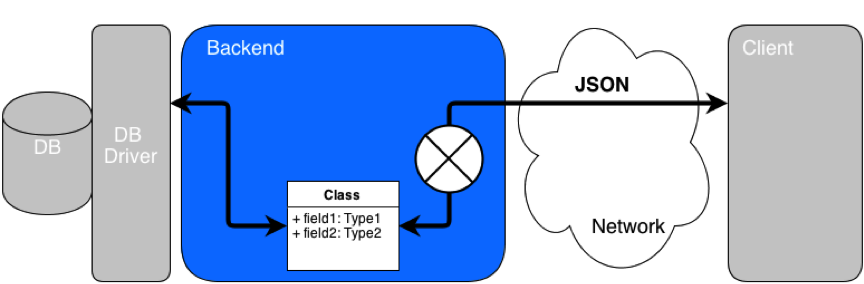
\includegraphics[width=0.8\textwidth]{img/orm.png}  
   \caption{Datenfluss einer Applikation bei Verwendung eines ORM Frameworks}   
  \label{fig:orm} 
\end{figure}

Der wichtigste Vorteil eines Frameworks für die objektrelationale Abbildung liegt in der Abstraktion von der Datenbank. Für die Business-Logik gibt es keinen Unterschied zwischen Objekten aus der Datenbank und Objekten der Programmiersprache. Die Datenbank kann meist ohne Änderungen an der Applikation ausgetauscht werden.

\FloatBarrier
\subsection{Objektrelationale Unverträglichkeit}

Ein ORM bringt konzeptionelle Probleme mit sich. Diese werden in der Literatur in der Regel als \tete{Object-relational Impedance Mismatch} (ORIM) bezeichnet. Die objektrelationale Unverträglichkeit resultiert aus den Unterschieden im zugrundeliegenden Konzept, sowie aus Differenzen in der Darstellung und den Erwartungen des Entwicklers \cite{bowers}.

Folgende Herausforderungen ergeben sich für die praktische Arbeit mit einem ORM:

\begin{itemize}
  \item Die Abbildung der Relationen zwischen den Objekten ist komplex. Es müssen One-to-One, One-to-Many und Many-to-Many Abhängikeiten ins relationale Schema übertragen werden.
\item Ein weiterer zentraler Punkt ist die Abbildung von Hierarchien und Vererbungen aus der objektorientierten Programmierung in das physische Datenmodell. 
\item Innerhalb des ORM muss es ein Objekt-Caching geben. Dieses ist notwendig um die Illusion zu erzeugen, dass es sich um ein Objekt der Programmiersprache handelt. Denn wird ein Objekt mehrmals aus der Datenbank abgefragt, so muss ein referenzgleiches Objekt zurückgegeben werden \cite{inappropriate-abstractions}.
\item Der Entwickler muss die ORM-Limitierungen, die sich aus dem ORIM ergeben, akzeptieren. Die Probleme müssen somit bekannt sein, um sie bereits bei der Datenmodellierung zu umgehen \cite{vietnam}. 
\end{itemize}

Ted Neward, Autor von „The Busy Java Developers Guide to Scala“, macht den frühen Erfolg von objektrelationalen Abbildungen und die Erleichterungen, welche die ersten ORMs mit sich brachten, dafür verantwortlich, dass zum Teil ORMs verwendet werden, ohne deren Limitationen zu beachten. Das wiederum führt zu Mehraufwand an Zeit und Energie für die Erhaltung und Anpassung an alle Nutzungsfälle \cite{vietnam}.

\subsection{Unterschiede zum data-centric Design}
Das data-centric Design ist viel stärker an die Datenbank gebunden und deren Austausch ist deutlich schwieriger. Dies sorgt dafür, dass keine Illusion einer abstrahierten Datenbank entsteht. Da das data-centric Design ein Ansatz mit funktionalem Hintergrund ist, sind die Datenstrukturen in der Regel unveränderbar. Ein Caching zur Sicherung der Objektidendität ist daher nicht notwendig. Die Objektgleichheit ist in diesem Fall über Wertgleichheit definiert (vgl. Scala Case Klassen \cite{scala-case-class}). Im Gegensatz zum ORM muss der Entwickler beim data-centric Design selbst um die Darstellung und Umwandlung seiner Daten in das Datenbankformat kümmern. Durch die Verwendung einer objekt- oder dokumentenbasierten Datenbank ist diese Umwandlung einfacher und mit weniger Problemen behaftet, als eine Konvertierung in ein relationales Schema.

\section{Abgrenzung zu Datenzugriffsobjekten}
Implementierungen von Datenzugriffsobjekten, in der englischsprachigen Literatur \tete{Data Access Object} (DAO) oder \tete{Data Access Procedure}, basieren auf dem \tete{Data Access Object} Pattern \cite{j2ee-pattern}.  Das Pattern hat das Ziel, den Datenzugriff und die Datenmanipulation in einen separaten Layer auszulagern. Daraus ergibt sich eine Kapselung der Datenbankzugriffe an einem Ort der Applikation. Bei der Umsetzung gibt es die Möglichkeit, ein DAO zur Abstraktion der Datenbank als Ganzes zu verwenden oder für jede einzelne Datenbankstruktur ein DAO anzulegen.

Der Hauptfokus liegt in der Abstrahierung der Datenbank. Bei Änderungen an der Datenquelle müssen in der Regel nur die Datenzugriffsobjekte angepasst werden, denn der Anwendungscode bleibt in der Regel unberührt. Die Serialisierung der Daten von den Strukturen der Anwendung in Strukturen der Datenbank ist nicht Aufgabe des DAO, sondern des \tete{Data Transfer Object} (DTO) \footnote{vgl. J2EE Patterns – Data Transfer Object \url{http://www.oracle.com/technetwork/java/transferobject-139757.html}}.

Im DAO findet über einen Datenbanktreiber direkter Zugriff auf die Datenbank statt. Man kann das Datenzugriffsobjekt somit als Bindeglied zwischen Datenbank und Applikation sehen. Durch die direkte Kommunikation mit der Datenquelle können alle unterstützten Funktionen ausgenutzt werden. 

Sowohl DAO als auch ORM haben die Abstrahierung der Datenbank als Ziel. Im Gegensatz zum DAO geht das ORM jedoch noch einen Schritt weiter und abstrahiert nicht nur über die Funktionen, welche durch die Datenbank zur Verfügung gestellt werden, sondern auch über die Innere Struktur der Datenquelle. In der Regel bauen ORM-Implementierungen auf dem Data Access Object Pattern und dem Data Transfer Object Pattern auf.

\subsection{Unterschiede zum data-centric Design}
Das DAO-Pattern enthält, ähnlich dem data-centric Design, keine Serialisierung oder Deserialisierung. Beide Designs können sehr gut zusammen verwendet werden. Der Datenfluss kann so durch ein DAO realisiert werden. Dadurch wird eine deutlich stärkere Kapselung erreicht. Voitet benutzt in seinen Beispielen kein DAO, sodass sich die Datenbankabfragen über den kompletten Quellcode verteilen. Während das bei Beispielapplikationen oder kleinen Anwendungen kein Problem darstellt, geht bei größeren Anwendungen mit vielen verschiedenen Datenmodellen schnell die Übersichtlichkeit verloren. Die Verwendung eines Datenzugriffsobjektes führt zu einem \tete{Single point of responsibility}\footnote{ Single responsibility prinziple (SRP), vgl. \cite[p.~339]{design-patterns}}
 und stärkt somit die Struktur des gesamten Projektes. 

\section{Grenzen des data-centric Designs}
Das data-centric Design eignet sich sehr gut für \tete{Create-Read-Update-Delete} (CRUD)-Anwendungen. Dort liegt der Fokus auf der Datenmanipulation, was zum Grundsatz des Designs passt.

Es erfolgt eine explizite Bindung an das Datenmodell. Durch die Nähe zur Datenquelle können spezifische Fähigkeiten einer Datenquelle genutzt und Anfragen effektiver gestaltet werden. Die dynamischen Strukturen des Datenmodells ermöglichen eine leichte Veränderbarkeit des Modells sowie einfache Verknüpfungen zwischen Daten.

Grenzen sind dem data-centric Design vor allem durch die Business-Logik gesetzt. Durch die dynamischen Strukturen im Design ist der Code meist komplizierter und länger.

Ohne die Verwendung eines DAO gibt es in diesem Design keinen Singe point of responsibility für Datenbankzugriffe. Das erschwert wiederum Änderungen am Schema, da diese zu unvorhergesehenen Problemen an anderen Stellen im Anwendungsquelltext führen können. Aus diesem Grund sollten bei diesem Design ein oder mehrere Datenzugriffsobjekte verwendet werden.

\section{Umsetzung in Project-Zoom}
Die REST-Schnittstelle von Project-Zoom entspricht die einer klassischen CRUD-Anwendung. Aufgrund der geringen Business-Logik liegt es nahe, das data-centric Design zu verwenden. Um die Wartung des Systems zu erleichtern, werden Datenzugriffsobjekte für jedes Datenmodell verwendet.

\lstinputlisting[caption=Macro Verwendung zur Generierung einer JSON Konvertierung, label=lst:json-format, language=scala]{code/json_reads.scala}

Für einige Teile der Anwendung ist es notwendig die JSON-Strukturen der Datenbank in Scala-Objekte umzuwandeln. Dies ist zum Beispiel für User Objekte der Fall, welche von der Authentifizierungsbibliothek SecureSocial verwendet werden. Play erlaubt die Generierung der Transformationsfunktionen mit Hilfe von Macros\footnote{JSON Macro incepetion \url{http://www.playframework.com/documentation/2.1.1/ScalaJsonInception}}. Das bedeutet, dass die Anwendung die Datenklassen des Modells definiert und die Funktionen zur Konvertierung von und nach JSON während der Kompilierung vom Framework übernommen werden. Ein Beispiel für solch eine Transformation ist in \ref{lst:json-format} mit der Variablen \tete{userFormat} gegeben. Diese ist in der Lage, zwischen den beispielhaften Repräsentationen 
\begin{lstlisting} 
{ 
  "firstName" : "Max", 
  "lastName"  : "Mustermann" 
}
\end{lstlisting} und 
\begin{lstlisting} 
User("Max", "Mustermann")
\end{lstlisting} 
zu konvertieren. Diese Bedarfskonvertierung ist durch die Verwendung von unveränderbaren Case-Klassen typsicher und entspricht den Konzepten der funktionalen Programmierung \cite{functional-thinking}.

Die CRUD-Operationen \tete{list} und \tete{read} wurden implementiert, ohne Datenbankobjekte zu konvertieren. Die Daten werden aus der Datenbank gelesen, transformiert und anschließend an den anfragenden Clienten zurückgegeben. Bei der Transformation werden z.B. Passwort-Hashes und Login-Informationen, die sich im User-Objekt befinden, entfernt. Die Funktionen \tete{create}, \tete{update} und \tete{delete} sind nicht für alle Datenbankobjekte implementiert. Dies liegt an der Anforderung, dass die Datenhaltung in der von der D-School bereits verwendeten Datenbank geschehen soll. Project-Zoom soll diese Daten nur aggregieren.
